\documentclass[a4paper, notitlepage]{article}
%\usepackage[cm]{fullpage}
\usepackage[pdftex]{graphicx}
\usepackage{wrapfig}


\begin{document}

\title{Data Management} 
\date{\today}
\maketitle


\section{Problem definition}

Our research showed that many of the algorithms require storage of data. We have identified the following types of data:

\begin{itemize}
	\item \textit{Raw data} - because of api restrictions
	\item \textit{User provided data}
	\item \textit{Intermediate results}
	\item \textit{Ready user profiles} - in order to be able to see how profiles are changing over time
	\item \textit{System data}
\end{itemize}

Problems:

\begin{itemize}
	\item Knowledge required - most have mathematical, statistical background
	\item Set up, maintain and admin(opened ports, firewalls, backup) db servers. Everyone has on setup and it is hard to manage.
	\item Change structure
	\item Collaboration and Access control(data structure and semantics is unknown)
	\item Low level queries
	\item RGL to native
\end{itemize}


\section{Challenges}

\begin{itemize}
	\item Multitenant storage with collaboration
	\item ORM of dynamic entities
	\item ORM fine grained access control
\end{itemize}

\section{Approach}
In this chapter we device a framework that is responsible to solve the Data management problem defined in the \textbf{requirements} section. By carefully analysing the requirements we concluded that the problem can be broken down into the following sub-problems:
\begin{itemize}
	\item \textit{Data storage and retrieval} - enable nested relational data oriented systems to hold their long-term data safely in a database and access it when needed.
	\item \textit{Multitenancy} - enable multiple users to work simultaniously with the solution and enable them to collaborate together in secure fashion.
	\item \textit{RDFGears extension} - extend the rgl engine and execution engine so that the system is able to deal with this new type of functionality correctly and efficiently.
\end{itemize}

Next subsections explain how each of the sub-problem is approached and solved.

\subsection{What do we want to store?}

\textbf{Define what is entity}

From section \textbf{problem def} makes clear that users' needs vary greatly and are likely to change in future. It is next to impossible to predict and define the structure and semantics of all data that users might like to store. Therefore, a more generic solution is needed. Users should be able to define the semantics and structure of the data they want to store on demand. This structure has to be able to be adapted over time if/when users' needs change. The solution has to be able to deal with all defined "entities" in uniform and predictable manner.   

All data in RDF Gears is presented in the RGL format and therefore the best approach is to provide users functionality that enables them to define these data entities in terms of RGL values. Once, this entities are defined the system should provide components that enable users to perform the needed operations over the data(CRUD) without any need for the users to know how the data is stored internally.

\subsection{Data storage and retrieval - How are we going to store and retrieve it? }

Once we have defined the structure of the data(predefined entities described in RGL) and the operations that has to be performed over the data(all CRUD operations) we have to provide solution that can cope with that. After rigorous research we did not find any existing solutions that can perform this operation. However, we discovered that Object/Relational Mapping (ORM) frameworks provide similar functionality to what we are looking for. Basically, they provide a methodology and mechanism for object-oriented systems to hold their long-term data(expressed as objects) in a relational database and later have it back in program objects when it is needed \cite{Neil}. ORM frameworks provide a level of abstraction over the process of storing data and in this way users can think(store, query) of the data as objects and they are not require to know details about the underling representation of the data. 

Therefore, applying the same approach for our RGL entities will completely satisfy our requirements for simplicity(users do not have to care about how data is stored). However, in order to do that we have two options. The first one is to implement and ORM solution from scratch and the other one is to extend/adapt existing ORM solution so that it is able to deal if RGL entities. In general, reusing a popular and widely used solution might be beneficial because it is likely it is heavily tested(at least from the engineers using it) and thus provide higher quality. 

Our research reviled that the Java Persistence Architecture API (JPA) is the "de facto" leader in the field ORM solutions for Java. It represents a Java specification(JSR 317) for accessing, persisting, and managing data between Java objects / classes and a relational database. Making its way as a major standard has resulted in a lot of the big players in the field providing an implementation of it. The most popular include: Hibernate(JBoss), TopLink (Oracle), EclipseLink(IBM) and openJPA(Apache). 

Because of its popularity, widely usage and formal standardization using the jpa  seems like the best option for our solution. However, in order to be able to use jpa we have to solve several major problems which are discussed in next sections.


\subsubsection{Express RGL in terms of JPA}
RDFGears already maps the RGL values to java objects. So the challenge is to map these classes to JPA in a sensible and efficient way. \textbf{Fig shows the classes organization}. The naive approach would be to reuse this structure directly. In this way each of the classes is represented as a separate entity. The main advantage of this approach is that the structure is fixed and it does not depend on the structure of the entities that we want to store. However, this approach also brings a lot of disadvantages. 

\begin{itemize}
	\item all data is in just several tables. This is inefficient and hard to scale.
	\item entities do not have names and they are hard to locate and query
	\item structure of the data/queries is not enforced and has to be explicitly validated
	\item changing structure may leave the db in inconsistent state
	\item hard to apply access control
	\item locs and transactions
\end{itemize}

The alternative approach that we propose is to map each entity into separate JPA entity which is named after the name of the entity(has to be unique). Table \textbf{tbl} proposes a methodology to map RGL values to JPA entities. 

\begin{center}
    \begin{tabular}{ | l | l |}
    \hline
    RGL & JPA  \\ \hline
    Record & Entity  \\ \hline
    Bag & Bag  \\ \hline

    \end{tabular}
\end{center}

This approach does not suffer from the problems of the first approach. However, it exposes several issues. The first thing is that each time the structure of an entity changes the JPA mapping and the schema of the underling db has to be changed. Our solution to this problem is discussed in the next section. The second thing is that JPA requires that each entity has distinct id but RGL does not provide such properties. We solve that problem by introducing auto generated ids for each entity which are made transparent to the client system(RDF Gears). Finally, entities must have distinct names. We solve this problem by making sure that each user defined entity has a unique name, and all record properties have distinct names. In order to make the names of sub-entities(records) distinct we append to the front of their name the full path from the root entity separated by "\_".


\subsubsection{Entities are virtual}
Once we know how to map the RGL entities to JPA entities we should enable jpa to deal with this RGL entities. However, JPA expects that each entity will have its own class representing it but our entities are virtual and are no java classes that represent them. One solution to this problem would be to generate this classes on runtime. However, this approach is complex and error prone. Therefore, we continued our research for simpler approach. We discovered a promising feature in hibernate called "Dynamic models". It basically allows to define the orm logic into a mapping xml file and in run time present the data as java collections(Maps, Lists, Sets, etc.)\textbf{tbl RGL to collection}. Therefore, when an entity is defined we have to build the xml mapping file and on runtime convert the rgl entities into java collections and use jpa to store them into the database.

\begin{center}
    \begin{tabular}{ | l | l |}
    \hline
    RGL & Java collection  \\ \hline
    Record & Map  \\ \hline
    Bag & List  \\ \hline

    \end{tabular}
\end{center}
 
\subsubsection{Entities are dynamic}
The problem that has to be solved concerns the dynamic nature of the entities. In our solutions we want to enable users to update them if this is required. Unfortunately, ORM frameworks are not good in dealing with such things. The problem is that whenever the structure changes not only the mapping xml file has to change but also the database schema. Some JPA providers provide simple tools for table generation problem(e.g. hibernate's hibernate.hbm2ddl.auto option) but they are not applicable(recreate the entire db) or not recommended in production mode(update). Therefore, in order to solve that problem reliably our solution provides implementation that is responsible to first update the mapping files and secondly update the structure of the database using JDBC statements.

\subsubsection{Operations}
We have to identify how each of the CRUD operations is performed. The solution provides a RDF Gears component that is responsible to enable the user to configure and execute each type of the supported operations and convert RGL to JPA and vice versa.
\begin{itemize}
	\item create - this is operations inserts and entity into the database. The user has to provide the name of the entity that has to be stored and the data itself.
	\item read - JPA provides a special high level query language which ommits details about the internal representation of the stored data. Because of the direct mapping from rgl to jpa all possible operation on the predifiened entities makes sense. The only exception are the additional id field. In order to make it transparent to the users we will name it "\$id\$"(hibernate uses this notation to identify service fields) and using this field in queries will be forbidden.
	\item delete - normally in jpa is based on id, but since we do not have this in the semantics we provide an alternative approach. In this case users write a read query and all results(entities or sub entities) from the query are deleted. Users are responsible to make sure that the query will produce only the needed results
	\item update - like delete, update in jpa is also based on ids. So we approach the problem similarly the user writes a query that selects all entities(sub entities ) that will be updated. However, here we distinct two types of updates. The first one is to replace the value of a field(simple type, record or bag). The second one is responsible to add element into a bag.
\end{itemize}

\subsection{Multitenancy - How to enable multiple users to use the solution and collaborate?}
The second main challenges that we have to solve is to enable multiple users to work with the solution simultaneously. In literature this is referred to as multi-tenancy. It has significantly increased its popularity in recent years as a results of the advancements in cloud computing and database as a service in particular \cite{Hui}. 

Designing the solution we have to take into account the following things: how to organize the data into the database, how to enable collaboration and how to manage access control.

\paragraph{Database organization}
There are three main approaches for designing multi-tennant solution \cite{Hui}:

\begin{itemize}
	\item \textit{Independent Databases and Independent Database Instances (IDII)} - in this approach users share only the hardware(server). For each user an independent database instance is running. This approach provides good data isolation and security but maintenance cost is significantly increased as a result of the multiple running instances. Additionally, collaboration between engineers is problematic because of the difficulty to execute queries on data that is spread over several databases.  
	
	\item \textit{Independent Tables and Shared Database Instances (ITSI)} - in this approach users share the hardware but also the database instance. Each user has private tables(user id is usually appended at the beginning of the table name \cite{Hui}). This approach reduces the maintenance cost but still the number of tables increases linearly with the number of users. Collaboration is facilitated but querying data relating all users he has to union the data from all user tables. Another disadvantage of this approach is that because the tables are different for each user we also need a separate JPA mapping for each user with increases complexity additionally.
	
	\item \textit{Shared Tables and Shared Database Instances (STSI)} - in this approach, all users share the db instances as well as the tables. In this approach the number of tables does not increase when the number of users increase. As a result the maintenance cost is reduced, queering is simplified(no unions required) and JPA mapping is straight forward. However, this approach has some disadvantages. First, engineers are responsible to maintain the required level of isolation between different users(usually a column indicating the owner of the data is required and additional where clause when querying for particular user). Second, tables contain the data for all users which may lead to decrease of performance.
	
\end{itemize}

Discussing the advantages and disadvantages of all the approaches above, we decided to use the STSI because it is easy to map to JPA, enables collaboration, simplifies querying and is easier to maintain.    

\paragraph{Collaboration}
The ability for engineers building workflows to collaborate and reuse each others data is essential. Choosing STSI organization makes it easy for engineers to work with the data of the others. However, there are several issues that has to be discussed and addressed:

\begin{itemize}

	\item \textit{privacy} - sometimes users might not want others to use their data. This might be because of a privacy issues or entities are not designed to be shared. Additionally, engineers might want to limit the access to the data. For example they might only allow others to read the data but not to modify it. Therefore, when the engineer defines an entity he should be able to specify its sharing options which are enforced by the solution.
	 
	\item \textit{semantics and structure of shared data} - the solution can further assist engineers that want to reuse shared data by providing information about its structure and semantics. Implementing such functionality will save them a lot of time since otherwise this information has to be communicate by other means which may take a lot of time.
	
	\item \textit{entities mutation} - introducing the multi tenancy feature introduces the problem with the consistency. By design entities can change and evolve over time. Therefore the system should prevent any inconsistent results produced if the structure changes at the time a workflow is executed. Our solution deals with that problem using transactions. All data operations are executed in transactions which temporary lock the tables for modification. As a result, the changing request will wait for the tables to be released before applying the updates to the database schema.
\end{itemize}


\paragraph{Access control}

The solution has to be able to enforce the sharing options of the entities and make sure that data is not accessed illegally. Therefore, the solution provides access control functionality that is responsible to enforce this policies. Basically, jpa is not good at doing this, it does not provide any access control functionality out of the box(\textbf{check that}). Therefore, there are two possible places to put the access control logic. 

\begin{itemize}
	\item \textit{above JPA} - our solution wraps arround the JPA engine and thus, we can control all the requests that it receives. We can provide functionality that validates if the user has the needed permissions to execute that functionality. However, from engineering perspective doing this will be hard since JPA(JPQL) allowes engineers to consrtuct relatively complex queries and building a functionality that pareses this queries is not a trivial job to do which significantly increases the risk of security wholes.
	
	\item \textit{underling DB} - the second option is to make the database enforce the security policies. We think that this approach is much easier because database already provide sophisticated fine grained access control mechanisms(\textbf{cite needed}). The only think that we have do is to translate the security policy of our solution to the database language(DDL) and set them when an entity is created or modified. As a result, the database will stop the JPA accessing data that it is not authorised to access.
\end{itemize}

\subsection{RDFGears extension - How to enable RDFGears to work with this new kind of functionality?}
what side effects

To understand the problem this new components introduce we first have to understand how RDFGears work. 
how rdfgears works

rdfgears does not have any or branching and therefore it is expected that all components are executed. However, in order to improve efficiency it introduces some optimizations:
\begin{itemize}
	\item the engine compiles the workflow into a datastructure which contains the output node and all components that the output directly or indirectly depends on. Therefore, components that do not have (indirect) connection to the output node are omitted. This makes sense because the assumption is that components do not have any side effects and if they do not contribute for the final result then there is no difference if they are executed or not.
	
	\item the engine takes the output node and recursively executes all components which outputs are needed for the execution.
	  
	\item the results produced by a component are cached. Therefore, if their output is needed in several branches the value is calculated only once.
	
	\item iterations ...  
\end{itemize}

The problem is that our solution imposes on this optimizations is that the assumption that components do not have side affects is no longer correct. Therefore, the engine will not longer perform its tasks correctly. The trivial approach would be to simply remove all these optimizations but this is not a good idea because efficiency will suffer continuously. Therefore, we propose an alternative approach which aims to make the engine perform correctly but also keep the efficiency.

Our solution consists of the following steps:
\begin{itemize}
	\item extend the function description notation so that the engine knows if a component has side effects or not
	\item when the datastcutrure of the functions is built we also include the components that have side effects and recusivly all the components that they depend on.
	\item we perform all the optimizations to the output node(as it is currently done) as well as to all components with side effects. 
	\item when the workflow is executed we execute it for the output node and for all components with side effects. The caching mechanism prevents components to execute several times. The output of the workflow is still the output of the output node.
\end{itemize}

These steps ensure that all components with side effects are executed and the execution is efficient because all the optimizations are applied.

\section{Architecture}
We have already discussed the main problems that our solution is facing and the approach we will use to solve each of them. In this chapter we discuss the architecture of the solution.

\subsection{Context View}

\begin{figure}[h!]
  \centering
  	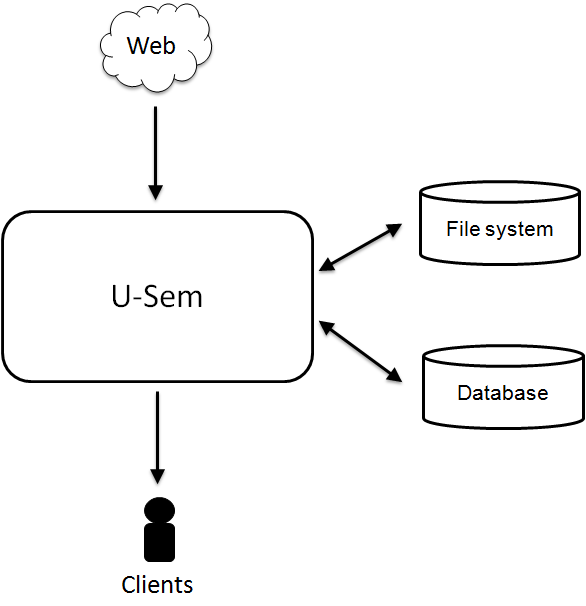
\includegraphics[scale=0.4]{environment/runtime_environment_storage.png}
  \caption{Context diagram of U-Sem }
  \label{fig_context}
\end{figure}

\subsection{Functional View}

\section{Implementation}

updated optimazer of execution engine to deal with side effects

\section{Evaluation and Future work}

Future work:
\begin{itemize}
\item transactions
\item caching echecache
\item better mechanism for changes of the database(might be solved by the transactions)
\item scalability
\end{itemize}

\begin{thebibliography}{99}

\bibitem{Neil} Object/Relational Mapping 2008: Hibernate and the Entity Data Model (EDM)

\bibitem{Hui} Supporting Database Applications as a Service

\end{thebibliography}

\end{document}